\documentclass{article}
\usepackage{amsmath,graphicx}

\begin{document}
\section{notes}
SPP is trying to avoid data augmentation . But the latest one introducing it model more sophisticated system.
Terms:dropout,maxout network
Reducing filter size help to improve system.Increasing depth will help. 
\section{Multi-stage Hubel-Wiesel architecture}
In 1962, Hubel DH and Wiesel TN\cite{Hubel1962},\cite{Hubel1965a} was studied visual cortex of anaesthetized cats  with   spots of white light of various shapes. They classified the  cells in the visual system in to  simple,complex and hypercomplex . Simple cells are influenced  by the arrangement of  excitatory and inhibitory regions of the receptive field and  position of stimulus is important . This cells receives input from cells of the lateral geniculate nucleus(LGN), which is connected to retina. But the complex cells will responds to  a properly  oriented stimulus regardless of the cell position in the receptive field. Complex cells are activated by edge,dark bar,slit and mixed stimuli . Hypercomplex cells are activated by edge,single-stopped(corner),double-stopped (tongue),slit(double-stopped)and dark bar(double-stopped).

\par Hubel DH and Wiesel TN \cite{Hubel1965a} presented a functional hierarchical structure of the visual cortex . According to their model, visual perception cells are in the  order , $simple\Longrightarrow complex\Longrightarrow lower \ order  \ hypercomplex  \Longrightarrow higher \ order \ hypercomplex$. Activation of  lower stage is  influenced by  the position of the input patterns and  higher stages are  position-invariant. There are several  contradictory to this structure, but no one   completely deny this hierarchical model.
\par Inspired by this work  , Fukushima, K \cite{Stark1980} proposed a neural network model for pattern recognition called neocognitron.
In neocognitron , cells are arranged in  a number of  cascded structure. Each  structure $U$ include a  simple cell layer $U_s$ and a complex cell layer $U_c$. This network is not affected by change in position or small distortion in the shape of patterns.  It is also capable to do self organization based on an unsupervised competitive learning algorithm\cite{Fukushima1982} in the first two layers and classification based on  supervised learning in the output layer.
\begin{figure}[ht]
 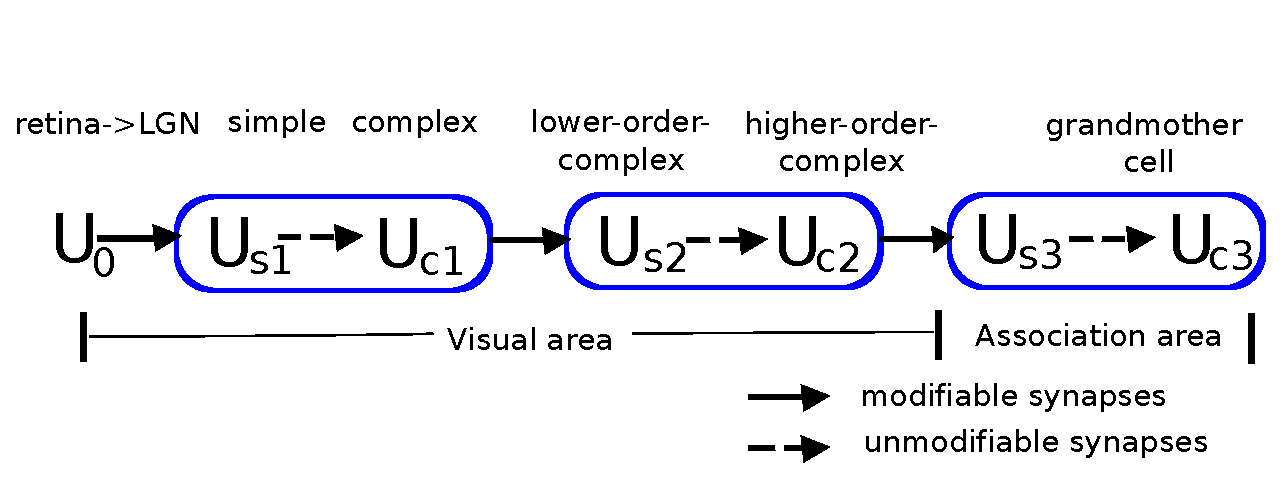
\includegraphics[]{Figures/neocognitron.eps}
\caption{Neocognitron\cite{Stark1980}}
\label{neo}
\end{figure}
\par This design was improved by  Yann LeCun \cite{lecun-86},\cite{lecun-89d}, \cite{lecun-89e},\cite{lecun-90c}, \cite{lecun-90e} using backpropagation algorithm\cite{BRYSON1963} to train the entire system.




%2012




%2013

\section{Network In Network }
Inspired by the work of Ian J. Goodfellow et al.\cite{Goodfellow2013} on maxout networks,  Min Lin et al.\cite{Lin2013} introduced a micro network in each convolution layer so that it will compute more abstract features.This network gave a state-of-the-art performance in  ILSVRC 2013 competition with an error rate of 12.95\%.They used NVIDIA TITAN GPU to train the newtork.

\section{Visualizing and Understanding Convolutional Networks}

Matthew D. Zeiler and Rob Fergus\cite{Zeiler2013} presented a method to visualize the function of intermediate feature layers of CNNs and used as a diagnostic tool to improve  the model proposed by Krizhevsky et al.\cite{Krizhevsky2012a}. This method helped  them  to understand  activation in the feature maps with respect to the input patterns. It shows Krizhevsky et al.'s architecture does not have  enough mid frequency coverage in the first layer filters and aliasing artifacts caused by  large stride in the first layer convolutions. Authors solved this problems by decreasing filter size to $7\times7$ and reducing stride to 2.This implementation won the  ILSVRC 2013 competition with an error rate of 11.74\%


%2014

\section{Spatial pyramid pooling in Deep Convolutional Networks}
Instead of using fixed input size in CNNs, Kaiming He et al.\cite{He2014} suggested  the use of a spooling strategy called  spatial pyramid pooling(SPP)\cite{Grauman2005}\cite{1641019} to avoid cropping or warping of  images. It introduced a new layer on top of the convolution layer and perform aggregation  based on Bag-of-Words (BoW) model \cite{Sivic2003}. But the classical back propagation training methods expect layers to have a fixed   size. To overcome this problem author implemented two fixed size networks with shared parameters and switch the network on alternate epochs. This network is trained using a single GeForce GTX Titan GPU with a starting  learning rate of 0.01 and achieved  a less  error rate of 8.06\% on  ILSVRC 2014 data set. 
\par 
This implementation improves the performance of baseline architectures including ZF-5\cite{Zeiler2013} , Convnet \cite{Krizhevsky2012a} and Overfeat-5/7 \cite{Sermanet2013}. Their study shows, accuracy of CNNs will improve on multi-size training, multi-level pooling, and full-image representations. 
%




\section{Going deeper with convolutions }
Christian Szegedy and et al.\cite{Szegedy} proposed a network named GoogLeNet with receptive field(input layer) of size $244\times244$ with the number of layers around 100. Network is trained using asynchronous stochastic gradient descent with 0.9 momentum and fixed learning rate schedule based on  no of epochs 
. Learning procedure took advantage of  model and data-parallelism in a CPU-based cluster environment. This network gave an error rate of  6.67\%  on  ILSVRC 2014 data set. Their result shows that use of existing dense  blocks to  build the sparse structure can improve the  performance of convolutional networks.


\section{VERY DEEP CONVOLUTIONAL NETWORKS FOR LARGE-SCALE IMAGE RECOGNITION}
Karen Simonyan and Andrew Zisserman \cite{Arge2015} evaluated the effect of network depth in image classification using very small convolution filters. Their deep network architecture comprise of fixed  size input layers , a stack of convolution layers , three Fully-Connected (FC) layers and  5 max-pooling layers for spatial spooling  over a $2 \times 2$ pixel window with stride 2. Hidden layers are modeled using Rectified Linear Units(ReLU)\cite{Nair2010}. On the hardware side, it uses a multi-GPU system with NVIDIA Titan Black GPUs. Network is trained using multinomial logistic regression  based on backpropagation with momentum of 0.9 and  batch size  256.
\par
 In this work authors formed a conclusion that greater depth with small convolution filters and  initialization of certain layers will cause the learning process to converge in less number  of epochs. This model of the convolution network does not differ from the classical architecture proposed by  LeCun et al.\cite{LeCun1998}. But the authors reported a significant improvement in the performance using an increased depth.  This implementation results in a significant improvement in accuracy with  an error rate of  6.8\% in  ILSVRC 2014 of ImageNet.

\begin{section}{Deep Image: Scaling up Image Recognition}
The latest attempt in image classification with an error 5.98\% in ImageNet data set is reported by  Ren Wu et al.\cite{Wu2015} of Baidu research.They developed an end to end deep learning  system named Deep Image. It uses a highly optimized parallel algorithm  to implement large deep neural network with augmented input data. The network is trained using stochastic gradient decent algorithms (SGD)[ref] on a custom built high performance system comprised of 36 server nodes, each with 2 six-core Intel Xeon E5-2620 processors and 4 NVIDIA Tesla K40m GPUs . System  uses an InfiniBand  network for interconnections. Parallelism strategies used in their network are model-data parallelism and data parallelism.  These methods have been proposed by Alex Krizhevsky \cite{Krizhevsky2014} and Omry Yadan et al.\cite{Yadan2013} for training convolutional neural networks with SGD on a  multiple GPU systems. But it is not easy extend the same strategies to multiple GPU clusters because of the communication overhead. So the  Baidu Team focused on minimizing network data transfers and overlapping the computation. They use butterfly synchronization and lazy update strategies to achieve data parallelism in the gradient computation. Their results show model-data parallelism is better when number of GPUs is less than 16. Implementation of Data parallelism in a large number  of GPU  cluster is better because of the constant communication requirements.
\par
The authors have explored different data augmentation techniques to increase the number of labeled images in the training set. This includes color casting, Vignetting, Lens distortion, Rotation, Flipping, and  Cropping. Instead of using the same resolution on all images, they have trained separate models at different scales, combined results by averaging soft max class posteriors.
Data set used in this experiment was subset of ImageNet dataset, used in the competition ImageNet Large-Scale Visual Recognition Challenge (ILSVRC)\cite{Berg2010}. This data set includes 1.2 million images which contain 1,000 categories.
\par
 Major contribution of this work is the demonstration of tremendous computational power to achieve high accuracy in image classification.
It also shows augmented multi-scale images can be combined to achieve less error rate in convolutional network in the context of the image classification. 
 \end{section}




\section{REFERENCES}
\label{sec:survey}
\bibliographystyle{IEEEbib}
\bibliography{survey}

\end{document}
